\documentclass[10pt,a4paper]{article}
\usepackage[utf8]{inputenc}
\usepackage{amsmath}
\usepackage{amsfonts}
\usepackage{amssymb}
\usepackage{graphicx}
\usepackage{geometry}
\geometry{
a4paper,
total={210mm,297mm},
left=20mm,
right=20mm,
top=20mm,
bottom=20mm,
hoffset=-10pt
}
\usepackage[varg]{txfonts}
\begin{document}
\title{Problems for Tutorial-03: Curve Fitting}
\date{}
\maketitle
\begin{enumerate}
\item Fit the data present in the file \verb'Tut3Problem.csv' to the function
\begin{align*}
	\mathcal{G} = \left(K + \omega \cos(t)\right)\sin(t), 
\end{align*}
where $K$ and $\omega$ are unknown. The first column 
in \verb'Tut3Problem.csv' is $t$ and the second column is the measured data. (Use least 
squares fitting).
\item Plot the measured data and fitted data versus $t$.
\end{enumerate}
{\bf Solution:}
\begin{figure}[ht!]
\raggedleft{
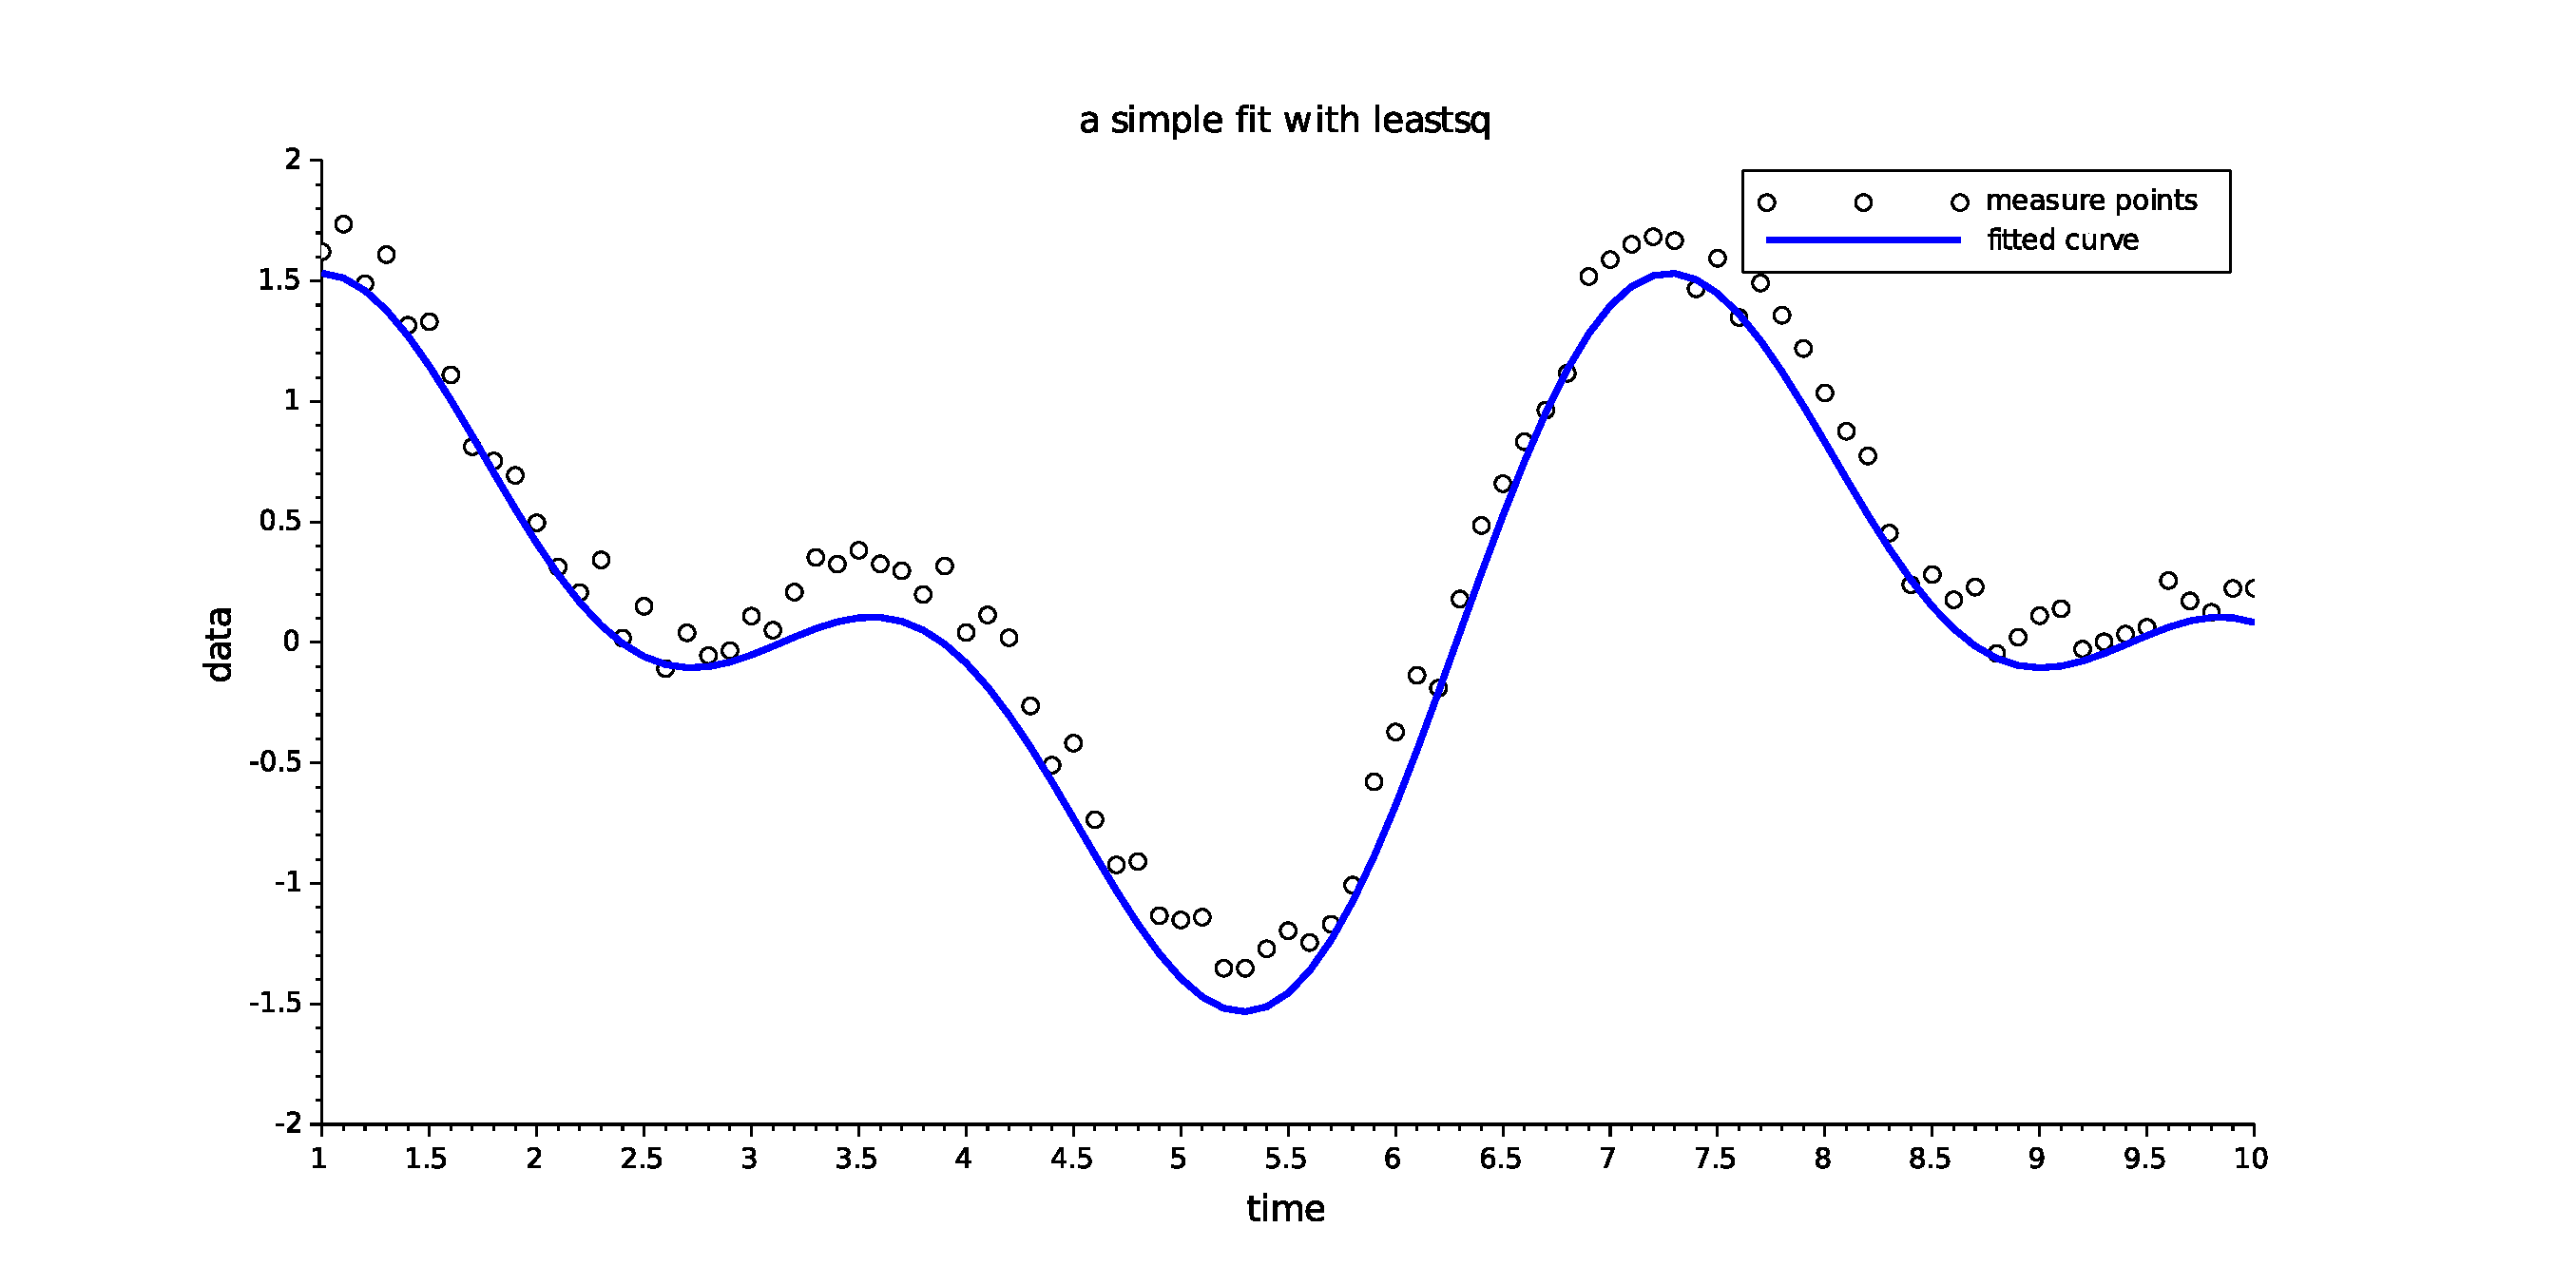
\includegraphics[scale=0.4]{SolPrblm03.pdf}}
\end{figure}
\end{document}
